%%%%%%%%%%%%%%%%%%%%%%%%%%%%%%%%%%%%%%%%%%%%%%%%%%%%%%%%%%%%%%%%%%%%%%%%%%%%%%%%
\section{Methodology/Design}
\label{sec:methodology}

Use this section describe the main contribution of your paper. If you are
building something, describe the design of the system you built. If you are
measuring something (like the world!) then include the measurement pipeline.

This is typically the largest section in your paper. (In case of measurement the
result section might be bigger.)


Make sure you give enough details so that the reader is able to reproduce your
work.

\subsection{Evaluation}
\begin{figure}
    \centering
    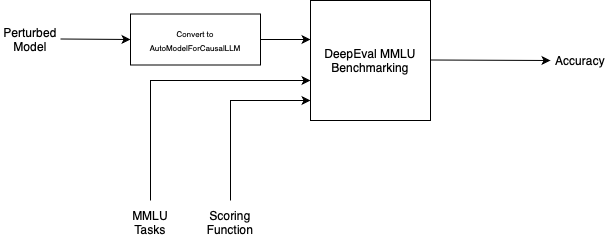
\includegraphics[width=1.0\linewidth]{Course Project Template//images/evaluation-pipeline.png}
    \caption{Evaluation Pipeline}
    \label{fig:eval-pipeline}
\end{figure}
\subsubsection{MMLU Benchmark}
We evaluate our perturbed models on the Massive Multitask Language Understanding (MMLU) Benchmark. The MMLU Benchmark contains 15908 questions over 57 subjects. The difficulty of the questions ranges from an elementary level to an advanced professional level\cite{hendrycks2021measuringmassivemultitasklanguage}. 

For our particular evaluation framework, we narrowed the scope of our evaluation to the High School Computer Science and Astronomy tasks. The scope was narrowed from 57 tasks to 2 tasks due to the excessive computational costs required to run 15908 instances of inference on each perturbed model. These particular tasks were chosen since they provide around average performance (\ref{fig:mmlu-tasks}) without exceeding the input token limit for GPT-2 and Mistral 7B.
\begin{figure}
        \centering
        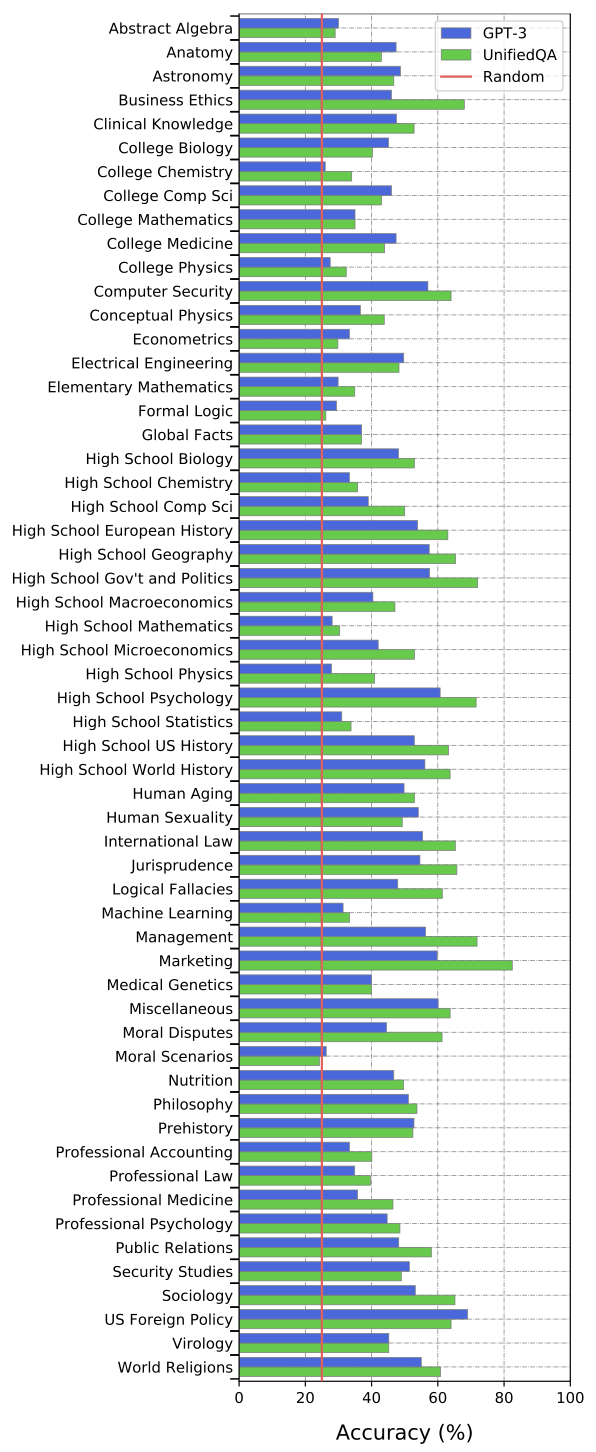
\includegraphics[width=0.75\linewidth]{Course Project Template//images/mmlu-task-performance.png}
        \caption{Performance of GPT-3, UnifiedQA and random guessing on all 57 MMLU tasks\cite{hendrycks2021measuringmassivemultitasklanguage}}
        \label{fig:mmlu-tasks}
\end{figure}

The evaluation was conducted in a 1-shot learning setup to isolate the effect of the perturbation on the model's intrinsic knowledge retention and generalization capabilities from few-shot learning. 

\subsubsection{DeepEval Testing Framework}
In order to standardize the evaluation of the perturbed models, we used an existing library in Python called DeepEval, an open-source toolkit for LLM evaluation. The framework consists of an inbuilt class to run evaluation on particular tasks of the MMLU benchmark. 

The MMLU Benchmarking class takes as input a model, and a set of tasks to run. It then uses the following algorithm to evaluate the model on the benchmark:
\begin{algorithm}
    \caption{Evaluation algorithm for model evaluation on MMLU}
    \label{alg:eval}
    \SetAlgoLined
    \KwIn{model, tasks, score\_fn}
    \KwOut{accuracy}
    \SetKwFunction{Evaluate}{evaluate}
    \SetKwProg{Fn}{Function}{:}{}
    \Fn{\Evaluate{model, tasks, score\_fn}}{
        total\_qs $\gets$ 0\;
        total\_correct $\gets$ 0\;
        \For{task \textbf{in} tasks}{
            golden $\gets$ dataset[task]\;
            \For{g \textbf{in} golden}{
                input $\gets$ format\_input(g)\;
                result $\gets$ model.generate(input)\;
                score $\gets$ score\_fn(result, g.answer)\;
                \If{score}{
                    total\_correct $\gets$ total\_correct + 1\;
                }
                total\_qs $\gets$ total\_qs + 1\;
            }
        }
        \Return total\_correct / total\_qs\;
}
\end{algorithm}
In \ref{alg:eval}, the function \verb|format_input| uses a specific template to format the input to instruct the LLM to correctly answer the question in a specific format. Also, \verb|model.generate()| refers to a generic function to generate output tokens from an LLM given some set of input tokens. 

\subsubsection{Exact Match Metric}
For this evaluation framework and benchmark, we use an exact-match metric. This is a popular metric that outputs a binary result where the input is penalized if it is not an exact match to the target. In this case, we compare the output token(s) to the target, and if it is not an exact match, we return \verb|false|.



